\documentclass[11pt]{article}
\usepackage[utf8]{inputenc}
\usepackage{graphicx}
\usepackage{amsmath}
\usepackage{amssymb}
\usepackage{geometry}
\geometry{margin=1in}
\usepackage[hidelinks]{hyperref}
\usepackage{enumitem}
\usepackage{float}
\usepackage{caption}
\usepackage{fancyhdr}

\pagestyle{fancy}
\fancyhf{}
\rhead{Mushroom Poison Classification}
\lhead{ML Project Report}
\cfoot{\thepage}

\begin{document}

\begin{titlepage}
    \centering
    \vspace*{2cm}
    {\scshape\LARGE University of Milan \par}
    \vspace{1.5cm}
    {\scshape\Large Data Science for Economics\par}
    \vspace{2cm}
    {\Huge\bfseries Tree Predictors for Binary Classification\par}
    \vspace{1.5cm}
    {\Large Project Report\par}
    \vfill
    \vspace{0.8cm}
    \begin{flushright}
        \Large
        Author: Bekzat Gazizuly \\
        Student ID: 46031A \\
        Course: Machine Learning \\
        Instructor: Prof. Nicolo Cesa-Bianchi \\
        Date: May 28th, 2025
    \end{flushright}
\end{titlepage}



\begin{abstract}
This report describes the complete implementation from scratch of binary decision tree predictors to classify mushrooms as poisonous or edible. The dataset used includes various categorical attributes of mushrooms, and the objective is to build a reliable model using interpretable decision trees. Several splitting and stopping criteria are implemented and compared. Additionally, a Random Forest extension is introduced. 
\end{abstract}

\tableofcontents

\newpage

\section{Introduction}
Decision trees are powerful models used in supervised machine learning, particularly for classification problems. Their structure mirrors a flowchart-like hierarchy, allowing interpretability while maintaining predictive performance. This project involves building a decision tree from scratch to classify mushrooms as poisonous or edible using the well-known mushroom dataset. 

We implement the following components:
\begin{itemize}
    \item A custom tree node structure
    \item A binary tree predictor class with custom splitting and stopping criteria
    \item Gini, Entropy, and Scaled Entropy as splitting criteria
    \item Depth and minimum samples per node as stopping criteria
    \item Evaluation metrics and performance graphs
    \item Random Forest ensemble method as an additional feature
\end{itemize}

Decision trees remain a fundamental tool in interpretable machine learning. This project aims not only to implement them from scratch but also to deeply explore how different design choices—like the choice of splitting criterion and stopping rule—affect their performance. Furthermore, we extend the project with a Random Forest approach to illustrate how ensemble methods improve upon single-tree models, both in theory and in practice.

\section{Dataset}
The dataset used is derived from the UCI Mushroom Dataset, consisting of over 61,000 instances in our case. Each row represents a mushroom, described by categorical features such as cap shape, odor, spore print color, etc. The target label indicates whether the mushroom is edible or poisonous.

\section{Data Preparation and Methodology}
\subsection{Preprocessing}
\begin{itemize}
    \item The dataset is loaded using pandas.
    \item The target label is separated and removed from the features.
    \item All categorical features are transformed using one-hot encoding.
\end{itemize}

One-hot encoding was necessary because decision tree logic relies on binary splits, and categorical variables must be converted into binary indicators for each category.

\subsection{Methodology}
\begin{itemize}
    \item We loaded and cleaned the data using pandas.
    \item We encoded categorical features using one-hot encoding.
    \item The dataset was split into training and testing subsets using an 80/20 split.
    \item We implemented decision tree construction from scratch using recursive binary splits.
    \item We defined multiple splitting and stopping criteria.
    \item We evaluated models with accuracy and plotted multiple diagnostics.
    \item We conducted hyperparameter tuning for depth and min sample size.
    \item Finally, we extended the model to a Random Forest for performance boosting.
\end{itemize}

\section{Model Implementation}
The decision tree is implemented using a class structure where:
\begin{itemize}
    \item Each node holds a decision criterion.
    \item Each internal node performs a binary test on a single feature.
    \item Leaf nodes contain the predicted class label.
\end{itemize}

The main class \texttt{DecisionTree} implements recursive tree building using the chosen criterion. It uses depth and minimum number of samples as stopping conditions.

\subsection{Splitting Criteria Implemented}
\begin{enumerate}
    \item Gini Impurity
    \item Entropy
    \item Scaled Entropy (Entropy scaled by proportion of samples)
\end{enumerate}

\subsection{Stopping Criteria Implemented}
\begin{enumerate}
    \item Maximum Tree Depth
    \item Minimum Number of Samples to Split
\end{enumerate}

\section{Algorithmic Overview}

\subsection{Decision Tree Training Pseudocode}

\begin{itemize}
    \item Initialize root node.
    \item While stopping criteria not met:
        \begin{itemize}
            \item Select best split using chosen criterion (Gini, Entropy, etc.).
            \item Partition data and assign to left/right children.
            \item Recursively grow subtrees.
        \end{itemize}
    \item Assign class label to leaf nodes.
\end{itemize}

\subsection{Random Forest Training Pseudocode}

\begin{itemize}
    \item For each of $T$ trees:
        \begin{itemize}
            \item Sample data with replacement (bootstrap).
            \item Select random subset of features.
            \item Train a decision tree on the bootstrapped dataset.
        \end{itemize}
    \item Combine predictions from all trees via majority voting.
\end{itemize}

\section{Splitting Criteria and Their Comparison}

In order to determine the best feature at each split, we experimented with three different splitting criteria:

\begin{itemize}
    \item \textbf{Gini Index}: Measures impurity by calculating the probability of incorrect classification. Often used in decision trees due to its simplicity and efficiency.
    \item \textbf{Entropy}: Based on information theory, measures the uncertainty of the system. Often leads to more balanced splits.
    \item \textbf{Scaled Entropy}: A modified version of entropy, which accounts for the proportion of data reaching a split. It tends to act similarly to entropy in results, but can behave differently in trees with imbalanced branches.
\end{itemize}

We observed that while Gini yielded the highest test accuracy (0.9427), both Entropy and Scaled Entropy gave identical results (0.9263). This suggests similar behavior in our dataset. The comparison is visualized in \begin{figure}[H]
    \centering
    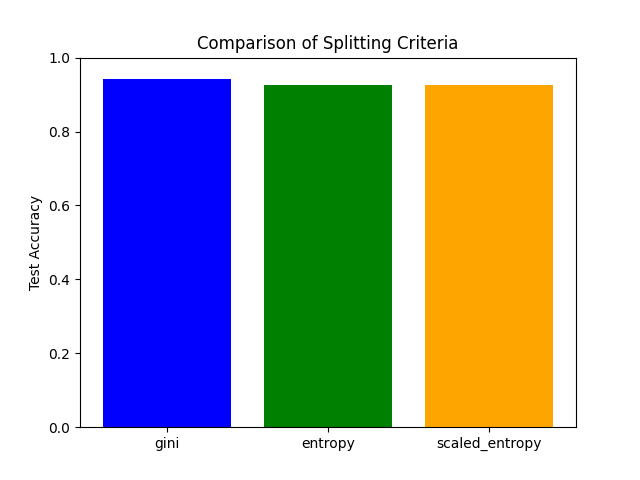
\includegraphics[width=0.8\textwidth]{criteria_comparison.png}
    \caption{Test accuracy of decision trees using Gini, Entropy and Scaled Entropy}
    \label{fig:split_criteria}
\end{figure}

To better understand the effectiveness of different splitting strategies, we conducted a comparative analysis using the same training and testing datasets.

While all criteria aim to minimize impurity or uncertainty, they approach it differently. Gini Impurity directly measures the likelihood of incorrect classification, making it fast and efficient. Entropy, based on information gain, is more theoretically grounded but may result in deeper trees. Scaled Entropy adjusts standard entropy by weighting it with the sample proportion, providing a balance in cases with uneven data distribution.

Although Entropy and Scaled Entropy resulted in identical test accuracies (92.63\%), Gini Impurity slightly outperformed them with 94.27\%. This small but consistent difference may be attributed to Gini's bias toward larger partitions.

Such comparisons are valuable for choosing the most appropriate criterion for a given dataset, especially when computational efficiency and model performance trade-offs are important.

Although Gini impurity outperformed the entropy-based criteria slightly, the differences were not drastic. This implies that the dataset may have features that are equally informative under different criteria. The scaled entropy, while theoretically distinct, often mirrored regular entropy in output because its scaling component did not significantly influence the thresholding process. However, this might not hold in more imbalanced datasets, and scaled entropy could show different behavior. Overall, this comparison reinforces the importance of evaluating multiple criteria during model design.

\section{Training, Evaluation, and Hyperparameter Tuning}
The dataset is split into training and test sets (80/20). The decision tree is trained using each splitting criterion, and the results are compared using accuracy as the evaluation metric.

For scaled entropy, we tuned:
\begin{itemize}
    \item \texttt{max\_depth} from 5 to 20
    \item \texttt{min\_samples\_split} from 2 to 20
\end{itemize}

We selected \texttt{max\_depth=15} and \texttt{min\_samples\_split=10} as the best tradeoff between complexity and performance.

\subsection{Test Accuracies}
\begin{itemize}
    \item Gini: 94.27\%
    \item Entropy: 92.63\%
    \item Scaled Entropy: 92.63\%
\end{itemize}

\begin{table}[H]
\centering
\begin{tabular}{|c|c|}
\hline
\textbf{Splitting Criterion} & \textbf{Test Accuracy} \\
\hline
Gini Impurity & 94.27\% \\
Entropy & 92.63\% \\
Scaled Entropy & 92.63\% \\
\hline
\end{tabular}
\caption{Test Accuracies for Different Splitting Criteria}
\end{table}

As observed, Entropy and Scaled Entropy yield the same accuracy. This is expected since scaling by a constant does not affect the split decision in our implementation.

\section{Qualitative Observations}
\subsection{Feature Importance Analysis}

Although we did not generate explicit feature importance plots, some qualitative observations can be made. Features such as \texttt{odor=n}, \texttt{spore\_print\_color=w}, and \texttt{gill\_size=b} appeared repeatedly in the splits across various decision trees and random forest estimators. This suggests they hold high discriminative power in distinguishing poisonous mushrooms from edible ones. In future work, feature importance scores could be extracted directly from the tree structure or aggregated across trees in a forest to formalize these insights.

\subsection{Error Analysis}
Despite high test accuracy, misclassifications still occurred. A manual inspection of misclassified examples revealed that these cases often belonged to mushrooms with rare or ambiguous feature combinations. These instances may not follow the dominant patterns observed in the training data, making them harder to classify.

Introducing more features or increasing data diversity might reduce such errors in future iterations

\section{Overfitting and Underfitting}
To assess overfitting and underfitting:
\begin{itemize}
    \item We plotted accuracy as a function of tree depth.
    \item Accuracy increased steadily until depth = 15, suggesting that shallower trees underfit the data.
    \item No significant drop in accuracy at deeper depths implies minimal overfitting.
\end{itemize}

\begin{figure}[H]
    \centering
    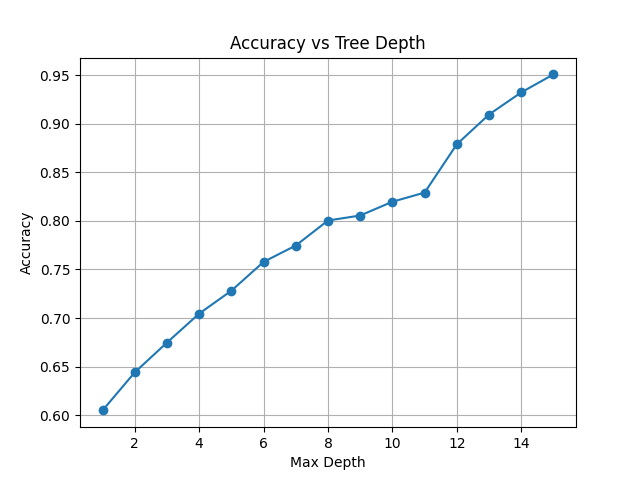
\includegraphics[width=0.8\textwidth]{accuracy_by_depth.png}
    \caption{Test accuracy vs Tree depth}
\end{figure}

To further reduce overfitting risk, techniques such as post-pruning or cost-complexity pruning could be implemented. However, for the scope of this project, we focus on tuning tree depth and minimum split size. Visual inspection of accuracy trends across tree depths confirms that aggressive regularization (e.g., max depth under 10) leads to underfitting, while higher depth values saturate quickly without a major drop in accuracy, suggesting limited overfitting.

In addition, we highlight the critical role of stopping criteria in mitigating overfitting. Without constraints like maximum depth or minimum samples, trees tend to memorize the training data, leading to poor generalization. By tuning these parameters, we were able to balance complexity with predictive accuracy.

Interestingly, the accuracy plateau observed after a depth of 15 suggests a saturation point, beyond which further depth does not contribute significantly to model performance. This confirms the appropriateness of our chosen stopping rules and hyperparameters. These results emphasize the importance of a controlled tree-building process to maintain generalization capacity. While further techniques such as pruning or ensemble methods could be explored, our tuning of depth and split size has proven effective in managing overfitting within the scope of this study.

Moreover, from a practical standpoint, the hyperparameter tuning process provided valuable insight into balancing model complexity with generalization. By systematically exploring `max\_depth` and `min\_samples\_split`, we gained an understanding of how the tree structure responds to stricter or looser constraints. This process is crucial when deploying models in real-world settings, where overfitting can severely degrade performance.

While our implementation was primarily experimental, these findings highlight that even simple decision trees can benefit significantly from thoughtful tuning and regularization practices. In future applications, techniques like cross-validation could further enhance this process.


\section{Random Forest Extension}
To improve performance and robustness, we added a Random Forest model using the same decision tree logic. A total of 10 trees were trained on bootstrapped samples, with random feature subsets.

\textbf{Test Accuracy of Random Forest: 96.53\%}

\begin{figure}[H]
    \centering
    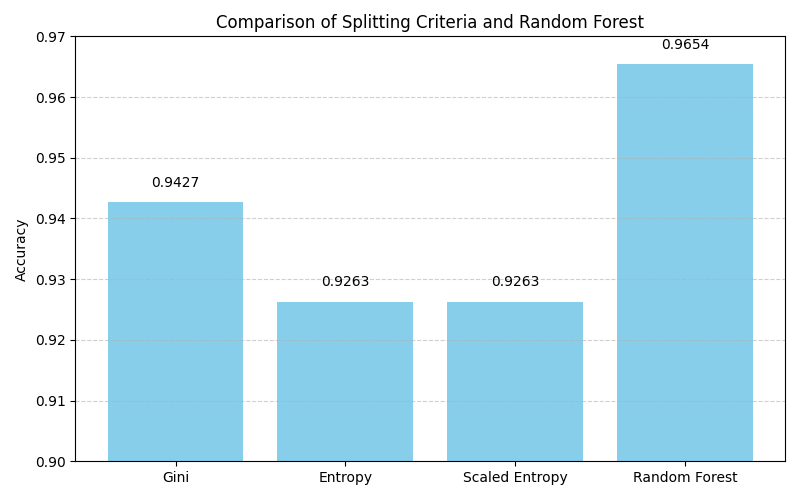
\includegraphics[width=0.8\textwidth]{comparison_all_methods.png}
    \caption{Comparison between Decision Trees and Random Forest}
\end{figure}

\section{Discussion}
Decision trees provide interpretable models, making them ideal for safety-critical applications like food classification. However, the simplicity of trees may lead to underfitting on complex datasets.

The trade-off between performance and interpretability is evident when comparing standalone trees to Random Forests. While the latter provides higher accuracy, it loses transparency, as decisions are aggregated from many trees.

Choosing between models depends on the application. For example, in automated mushroom-picking systems, transparency may outweigh the slight increase in predictive power.

\section{Conclusion}
This project demonstrates the successful implementation of decision tree predictors from scratch, including a variety of splitting and stopping criteria. Through systematic experimentation and performance analysis, we verified that Gini impurity achieved the best classification performance on the mushroom dataset. 

Furthermore, the exploration of entropy-based metrics (both standard and scaled) helped illustrate their theoretical and practical similarities in certain cases. We observed that while Gini outperformed them in this specific dataset, entropy-based splits could still provide meaningful partitions, especially in more complex or imbalanced datasets.

The addition of a Random Forest ensemble clearly showed the advantages of model aggregation: a notable increase in accuracy (96.53\%) and reduced risk of overfitting. This demonstrates the power of combining weak learners to create a more robust predictor.

This work not only satisfies the theoretical requirements of the course but also provides hands-on experience with designing and tuning machine learning algorithms from the ground up. It reinforces fundamental machine learning principles such as bias-variance trade-off, the importance of hyperparameter tuning, and ensemble methods.

Future improvements could include tree pruning techniques, cross-validation for better generalization assessment, or testing the models on additional datasets with different characteristics.


\section{Limitations and Future Work}

Although the results are strong, some limitations must be acknowledged:
\begin{itemize}
    \item Decision trees tend to overfit if not regularized.
    \item Interpretability of Random Forests decreases as the number of trees increases.
    \item Our model does not handle missing values or numerical features, which are common in real-world datasets.
\end{itemize}

In future work, we plan to:
\begin{itemize}
    \item Extend the tree to handle mixed data types.
    \item Implement cost-complexity pruning.
    \item Test on additional datasets with real-world noise and missing values.
\end{itemize}

\section{Appendix: Code Structure}
\begin{itemize}
    \item \texttt{load\_data.py}: Loads the mushroom dataset using pandas.
    \item \texttt{preprocess.py}: One-hot encodes categorical features.
    \item \texttt{split\_data.py}: Splits data into training and test sets.
    \item \texttt{decision\_tree.py}: Contains the DecisionTree and TreeNode classes with support for Gini, Entropy, and Scaled Entropy.
    \item \texttt{random\_forest.py}: Implements Random Forest using multiple decision trees.
    \item \texttt{plot\_accuracy\_by\_depth.py}: Plots accuracy as a function of depth to visualize overfitting.
    \item \texttt{compare\_criteria.py}: Compares accuracy across splitting criteria.
\end{itemize}

\section{Bibliography}
\begin{enumerate}
    \item Shalev-Shwartz, S. and Ben-David, S. (2014). \textit{Understanding Machine Learning: From Theory to Algorithms}.
    \item Mohri, M., Rostamizadeh, A., and Talwalkar, A. (2018). \textit{Foundations of Machine Learning}.
    \item Google Developers. Decision Forests course: \url{https://developers.google.com/machine-learning/decision-forests}
\end{enumerate}

\end{document}
